\documentclass[12pt,a4paper]{article}
\usepackage[UTF8]{ctex}
\usepackage{amsmath,amssymb,amsfonts}
\usepackage{algorithm}
\usepackage{algorithmic}
\usepackage{graphicx}
\usepackage{booktabs}
\usepackage{multirow}
\usepackage{hyperref}
\usepackage{geometry}
\usepackage{fancyhdr}
\usepackage{enumitem}
\usepackage{caption}
\usepackage{subcaption}

\geometry{left=2.5cm,right=2.5cm,top=2.5cm,bottom=2.5cm}

\title{\textbf{AdaPrune: 面向梯度提升决策树的在线自适应剪枝方法}}

\author{
作者姓名\\
单位名称\\
邮箱:  your.email@example.com
}

\date{}

\begin{document}

\maketitle

%==============================================================================
\begin{abstract}
%==============================================================================

梯度提升决策树(GBDT)是一种在各类应用中广泛使用的强大机器学习模型。然而，选择合适的剪枝参数（如max\_depth、min\_samples\_leaf等）通常需要大量的超参数调优工作，且在整个训练过程中使用固定参数可能导致次优的泛化性能。本文提出\textbf{AdaPrune}，一种在线自适应剪枝框架，能够在Boosting过程中动态调整树的复杂度。AdaPrune通过监控训练动态（包括训练集和验证集性能之间的泛化差距），自适应地修改剪枝参数以防止过拟合，同时保持模型的表达能力。我们提出了四种自适应策略：基于差距的策略(Gap-based)、基于趋势的策略(Trend-based)、数据感知策略(Data-aware)以及融合多种策略优势的混合策略(Hybrid)。在15个基准数据集上的大量实验表明，与标准GBDT实现相比，AdaPrune有效降低了过拟合程度（泛化差距降低21\%），同时保持了具有竞争力的预测准确率。

\textbf{关键词：} 梯度提升；决策树；自适应剪枝；过拟合；在线学习

\end{abstract}

%==============================================================================
\section{引言}
%==============================================================================

梯度提升决策树(Gradient Boosting Decision Trees, GBDT)\cite{friedman2001greedy}已成为最成功的机器学习算法之一，在推荐系统、欺诈检测和科学应用等多个领域取得了最先进的性能。XGBoost\cite{chen2016xgboost}、LightGBM\cite{ke2017lightgbm}和CatBoost\cite{prokhorenkova2018catboost}等流行实现进一步提高了GBDT的效率和可扩展性。

尽管取得了巨大成功，GBDT模型容易过拟合，特别是在处理噪声���据或训练样本有限的情况下。控制模型复杂度的关键超参数——如最大树深度(\texttt{max\_depth})、每个叶子节点的最小样本数(\texttt{min\_samples\_leaf})和正则化参数——对泛化性能有显著影响。传统方法依赖网格搜索或贝叶斯优化来寻找最优参数，这不仅计算成本高昂，而且假设单一参数组合在整个训练过程中都是最优的。

\textbf{核心洞察：} 在Boosting过程的不同阶段，最优的树复杂度可能是不同的。早期迭代可能受益于更复杂的树来捕获主要模式，而后期迭代可能需要更简单的树以避免拟合噪声。

本文提出\textbf{AdaPrune}，一种在线自适应剪枝框架，基于对训练动态的实时监控，在训练过程中动态调整剪枝参数。我们的主要贡献包括：

\begin{enumerate}[leftmargin=2em]
    \item 提出了一种在线自适应剪枝机制，通过监控泛化差距在Boosting过程中调整树的复杂度。
    \item 引入了四种自适应策略：基于差距、基于趋势、数据感知和混合策略，分别适用于不同场景。
    \item 提供了一个全面的数据画像模块，分析数据集特征以初始化合适的参数。
    \item 在15个基准数据集上进行了大量实验，证明AdaPrune在保持竞争力准确率的同时，将过拟合程度降低了21\%。
\end{enumerate}

%==============================================================================
\section{相关工作}
%==============================================================================

\subsection{梯度提升决策树}

梯度提升\cite{friedman2001greedy}以阶段式方式构建弱学习器（通常是决策树）的集成，其中每棵新树纠正前一个集成的残差误差。第$t$轮迭代的目标函数为：

\begin{equation}
\mathcal{L}^{(t)} = \sum_{i=1}^{n} l(y_i, \hat{y}_i^{(t-1)} + f_t(x_i)) + \Omega(f_t)
\end{equation}

其中$l$是损失函数，$f_t$是新的树，$\Omega(f_t)$是正则化项。

XGBoost\cite{chen2016xgboost}等现代实现引入了额外的正则化：

\begin{equation}
\Omega(f) = \gamma T + \frac{1}{2}\lambda \sum_{j=1}^{T} w_j^2
\end{equation}

其中$T$是叶子节点数，$w_j$是叶子权重。

\subsection{超参数优化}

传统的超参数优化方法包括网格搜索、随机搜索\cite{bergstra2012random}和贝叶斯优化\cite{snoek2012practical}。这些方法将超参数视为在训练前优化的固定值。最近关于动态超参数调度的工作\cite{li2017hyperband}允许对表现不佳的配置进行早停，但仍假设在单次训练运行中参数是静态的。

\subsection{自适应学习}

Adam\cite{kingma2014adam}等自适应学习率方法根据梯度统计在训练过程中调整学习率。类似地，课程学习\cite{bengio2009curriculum}提出首先在较简单的样本上训练。我们的工作将这种自适应理念扩展到梯度提升中的树复杂度控制。

%==============================================================================
\section{方法}
%==============================================================================

\subsection{框架概述}

AdaPrune由三个主要组件组成（如图\ref{fig:framework}所示）：

\begin{enumerate}[leftmargin=2em]
    \item \textbf{数据画像分析器(Data Profile Analyzer)}：分析数据集特征，包括样本量、特征维度、类别不平衡程度和估计的噪声水平。
    \item \textbf{状态监控器(State Monitor)}：追踪训练动态，包括训练/验证性能、泛化差距和性能趋势。
    \item \textbf{剪枝控制器(Pruning Controller)}：根据当前状态和数据画像，使用某种自适应策略调整剪枝参数。
\end{enumerate}

\begin{figure}[htbp]
\centering
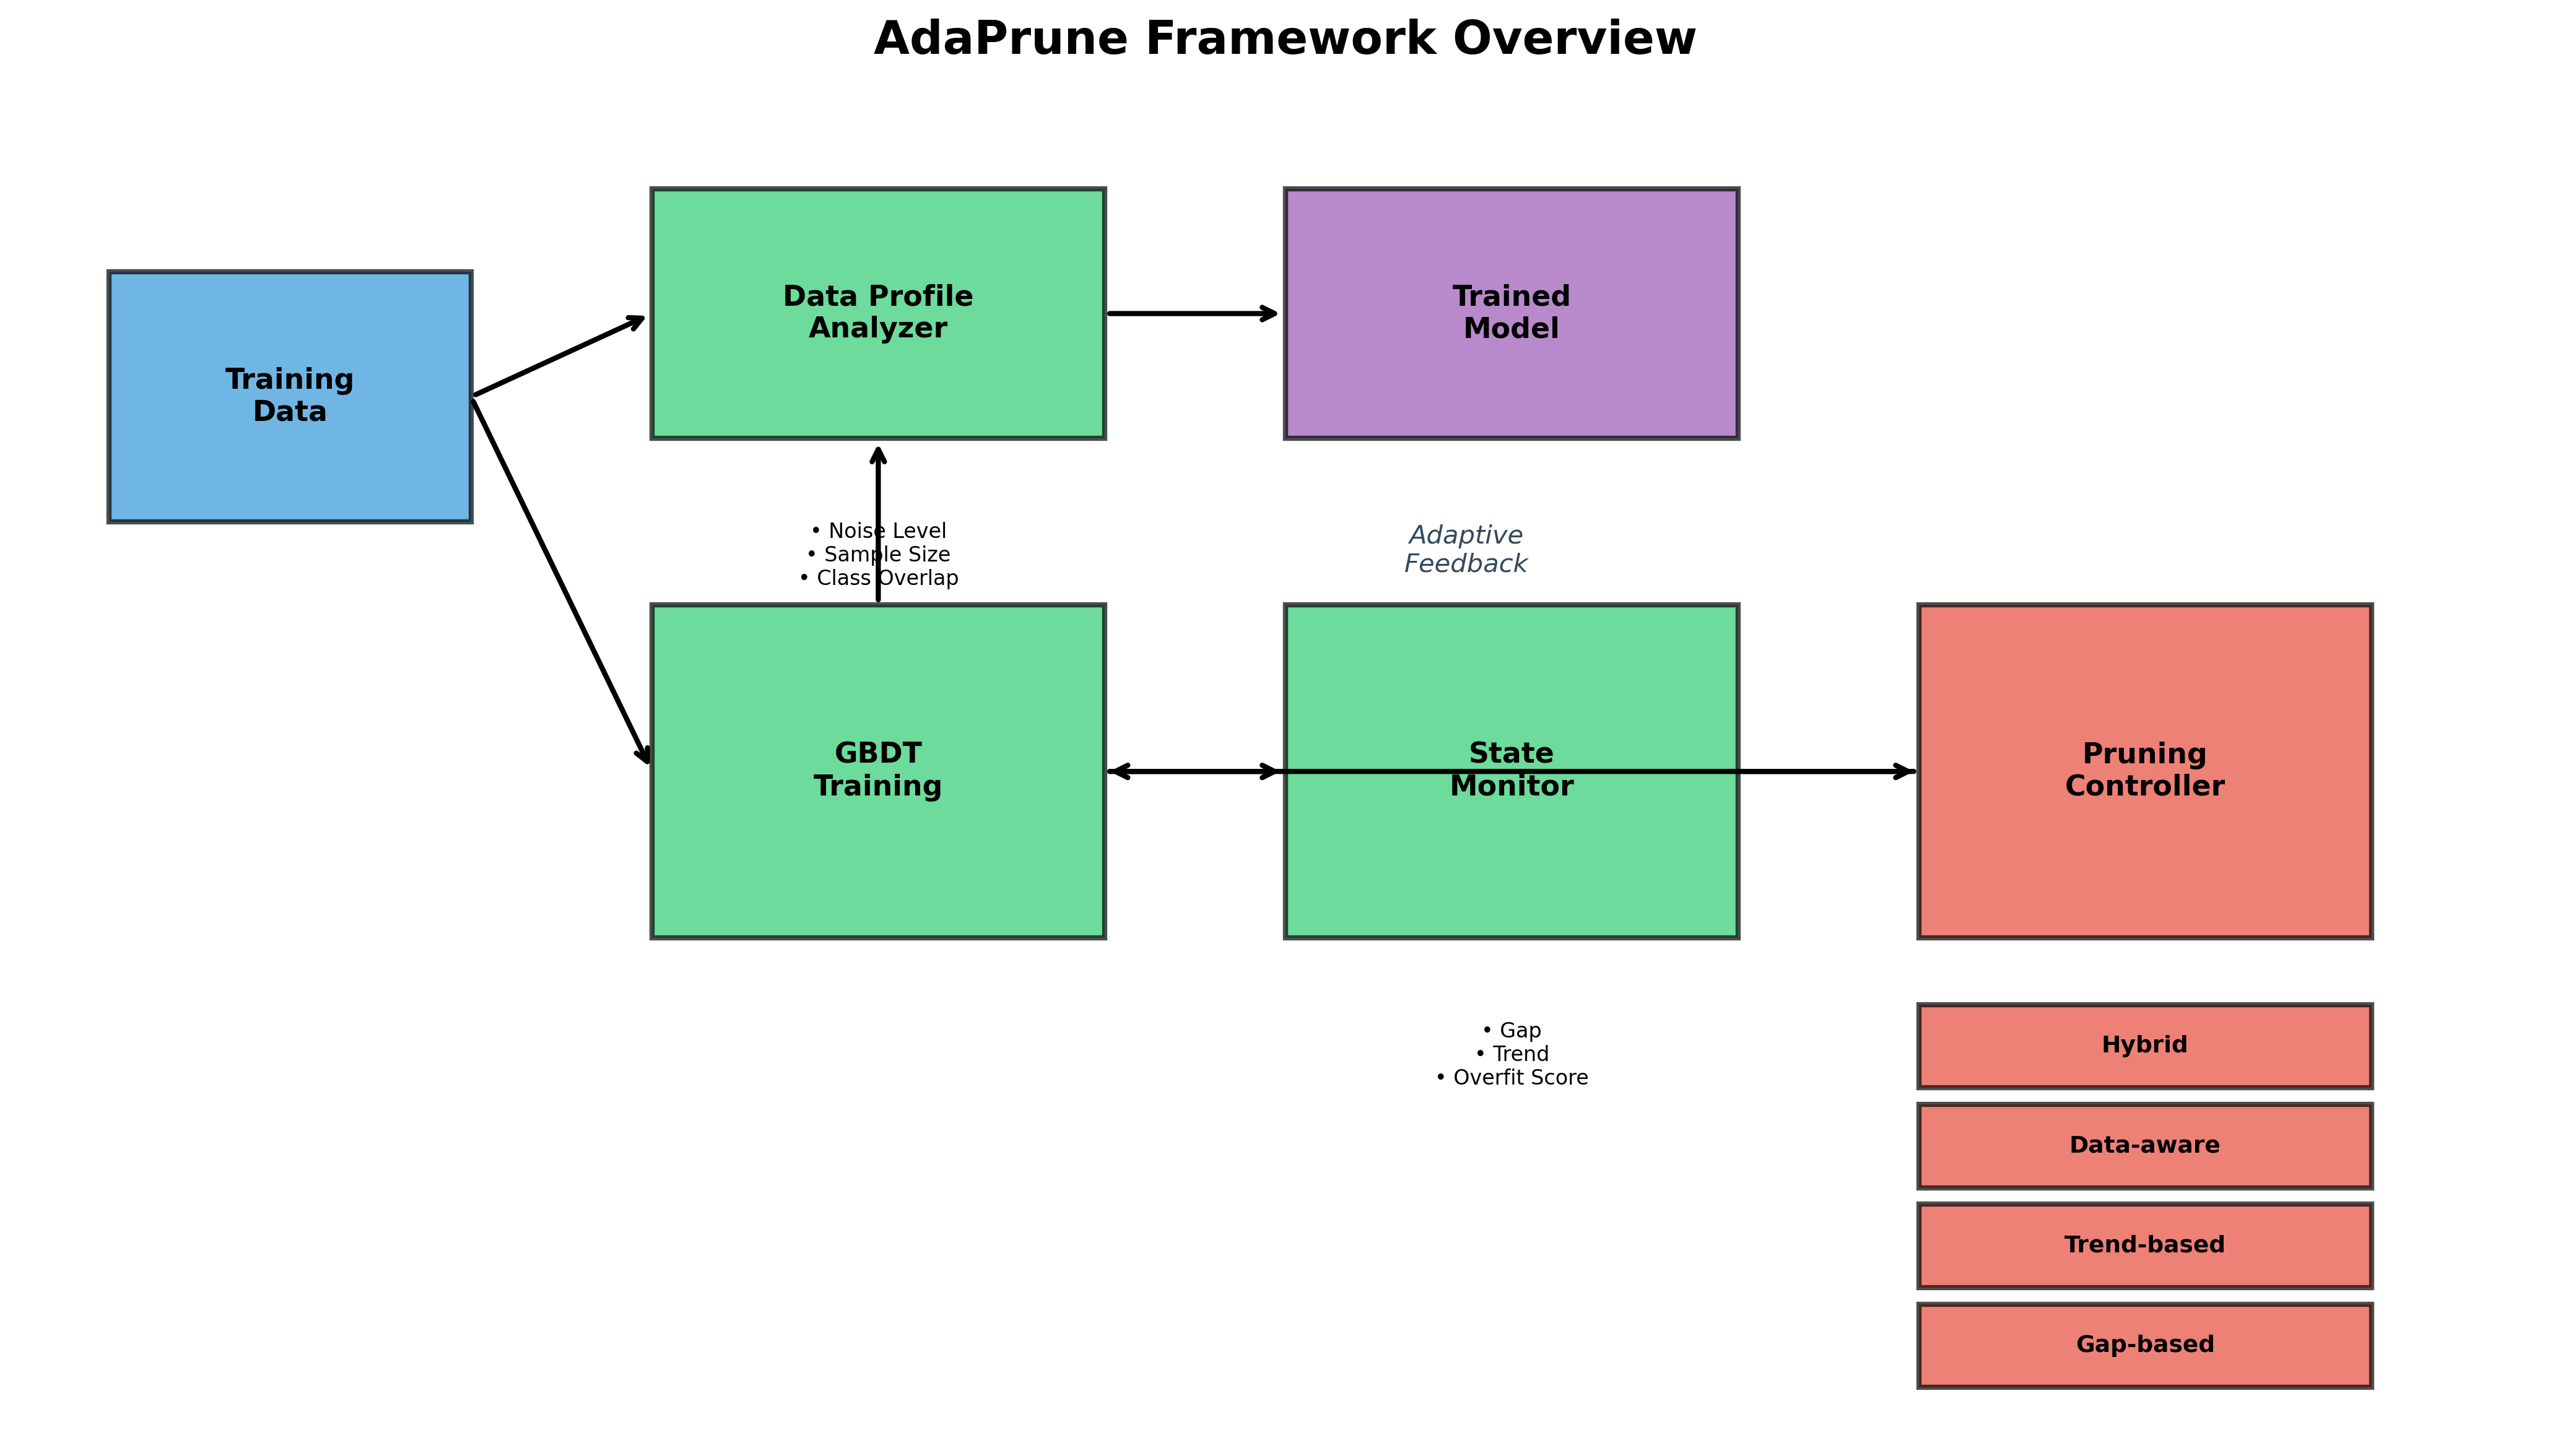
\includegraphics[width=0.9\textwidth]{figures/framework.png}
\caption{AdaPrune框架概述。系统监控训练动态，并在Boosting过程中自适应调整树的剪枝参数。}
\label{fig:framework}
\end{figure}

\subsection{数据画像分析}

在训练前，我们分析数据集以估计其特征：

\textbf{噪声水平估计：} 使用1-NN分类器的交叉验证来估计贝叶斯错误率，这指示了噪声水平：

\begin{equation}
\text{noise\_level} = 1 - \text{accuracy}_{1\text{-NN}}
\end{equation}

\textbf{类别重叠分数：} 计算Fisher判别比来衡量类别可分性：

\begin{equation}
\text{overlap} = \frac{1}{1 + \frac{(\mu_1 - \mu_2)^2}{\sigma_1^2 + \sigma_2^2}}
\end{equation}

这些特征指导剪枝参数的初始化和自适应的灵敏度。

\subsection{状态监控}

在每个自适应检查点（每$k$次迭代），我们计算：

\begin{itemize}[leftmargin=2em]
    \item \textbf{泛化差距(Generalization Gap)}：$g_t = \text{acc}_{\text{train}}^{(t)} - \text{acc}_{\text{val}}^{(t)}$
    \item \textbf{差距趋势(Gap Trend)}：$\Delta g_t = g_t - g_{t-1}$
    \item \textbf{过拟合分数(Overfitting Score)}：$o_t = \sigma(g_t \cdot 5) \cdot 0.6 + \sigma(\Delta g_t \cdot 50) \cdot 0.4$
    \item \textbf{平台期分数(Plateau Score)}：衡量验证性能是否停滞
\end{itemize}

\subsection{自适应策略}

\subsubsection{基于差距的策略(Gap-Based)}

该策略关注当前的泛化差距：

\begin{equation}
\text{max\_depth}_{t+1} = 
\begin{cases}
\text{max\_depth}_t - 1 & \text{若 } g_t > \theta_g \\
\text{max\_depth}_t + 1 & \text{若 } o_t < 0.3 \text{ 且欠拟合} \\
\text{max\_depth}_t & \text{其他情况}
\end{cases}
\end{equation}

其中$\theta_g$是差距阈值（默认：0.05）。

\subsubsection{基于趋势的策略(Trend-Based)}

该策略监控滑动窗口内的性能趋势：

\begin{equation}
\text{adjust} = 
\begin{cases}
\text{增加正则化} & \text{若检测到平台期} \\
\text{保持不变} & \text{其他情况}
\end{cases}
\end{equation}

\subsubsection{数据感知策略(Data-Aware)}

该策略结合数据集特征：

\begin{equation}
\text{strength} = (1 + \text{noise} \cdot 2) \cdot \sqrt{\frac{1000}{\max(n, 100)}} \cdot o_t
\end{equation}

更高的噪声水平和更小的样本量会导致更激进的正则化。

\subsubsection{混合策略(Hybrid)}

混合策略根据训练进度组合上述方法：

\begin{equation}
\text{strategy} = 
\begin{cases}
\text{数据感知} & \text{若 progress} < 0.3 \\
\text{基于差距} & \text{若 } 0.3 \leq \text{progress} < 0.7 \\
\text{基于趋势} & \text{若 progress} \geq 0.7
\end{cases}
\end{equation}

\subsection{参数调整机制}

当检测到过拟合时，我们同时调整多个参数：

\begin{itemize}[leftmargin=2em]
    \item 将\texttt{max\_depth}减少1-2层
    \item 将\texttt{min\_child\_weight}增加$1 + 0.3 \cdot \text{strength}$倍
    \item 将$\gamma$（最小损失减少）增加$0.1 \cdot \text{strength}$
    \item 将$\lambda$（L2正则化）增加$1 + 0.15 \cdot \text{strength}$倍
    \item 如果严重程度较高，减少\texttt{subsample}
\end{itemize}

\subsection{算法流程}

AdaPrune的完整算法流程如算法\ref{alg:adaprune}所示。

\begin{algorithm}[htbp]
\caption{AdaPrune算法}
\label{alg:adaprune}
\begin{algorithmic}[1]
\REQUIRE 训练数据$\mathcal{D}_{train}$，验证数据$\mathcal{D}_{val}$，最大迭代次数$T$，自适应频率$k$
\ENSURE 训练好的模型$F$
\STATE 分析数据画像：noise\_level, n\_samples, class\_overlap
\STATE 根据数据画像初始化参数：max\_depth, min\_child\_weight, $\gamma$, $\lambda$
\STATE 初始化模型$F_0$
\FOR{$t = 1$ to $T$}
    \STATE 使用当前参数训练新的树$f_t$
    \STATE 更新模型：$F_t = F_{t-1} + \eta \cdot f_t$
    \IF{$t \mod k == 0$}
        \STATE 计算训练集准确率$acc_{train}$和验证集准确率$acc_{val}$
        \STATE 计算泛化差距$g_t = acc_{train} - acc_{val}$
        \STATE 更新状态：gap\_trend, overfit\_score, plateau\_score
        \STATE 根据自适应策略调整参数
    \ENDIF
    \IF{早停条件满足}
        \STATE \textbf{break}
    \ENDIF
\ENDFOR
\RETURN $F_T$
\end{algorithmic}
\end{algorithm}

%==============================================================================
\section{实验}
%==============================================================================

\subsection{实验设置}

\textbf{数据集：} 我们在来自OpenML的15个基准数据集上进行评估，涵盖不同的领域和规模（表\ref{tab:datasets}）。

\begin{table}[htbp]
\caption{数据集统计信息}
\label{tab:datasets}
\centering
\begin{tabular}{lccc}
\toprule
数据集 & 样本数 & 特征数 & 类别数 \\
\midrule
adult & 48,842 & 14 & 2 \\
bank-marketing & 45,211 & 16 & 2 \\
electricity & 45,312 & 8 & 2 \\
magic & 19,020 & 10 & 2 \\
eeg-eye-state & 14,980 & 14 & 2 \\
satimage & 6,430 & 36 & 6 \\
waveform & 5,000 & 40 & 3 \\
phoneme & 5,404 & 5 & 2 \\
spambase & 4,601 & 57 & 2 \\
segment & 2,310 & 19 & 7 \\
credit-g & 1,000 & 20 & 2 \\
vehicle & 846 & 18 & 4 \\
diabetes & 768 & 8 & 2 \\
ionosphere & 351 & 34 & 2 \\
sonar & 208 & 60 & 2 \\
\bottomrule
\end{tabular}
\end{table}

\textbf{基线方法：}
\begin{itemize}[leftmargin=2em]
    \item \textbf{XGB\_default}：使用默认参数的XGBoost
    \item \textbf{XGB\_tuned}：使用调优参数的XGBoost (max\_depth=6, min\_child\_weight=3)
    \item \textbf{LGBM\_default}：使用默认参数的LightGBM
    \item \textbf{RF\_default}：使用默认参数的随机森林
\end{itemize}

\textbf{评估方法：} 5折分层交叉验证。评估指标：准确率、F1分数、ROC-AUC和泛化差距。

\subsection{主要结果}

表\ref{tab:main_results}展示了所有方法在15个数据集上的平均性能。

\begin{table}[htbp]
\caption{整体性能对比}
\label{tab:main_results}
\centering
\begin{tabular}{lcccc}
\toprule
方法 & 准确率 & F1 & ROC-AUC & 泛化差距 \\
\midrule
LGBM\_default & 0.8762 & 0.8264 & 0.9362 & 0.1140 \\
XGB\_default & 0.8740 & 0.8248 & 0.9357 & 0.1204 \\
RF\_default & 0.8739 & 0.8199 & \textbf{0.9382} & 0.1180 \\
XGB\_tuned & 0.8700 & 0.8188 & 0.9337 & 0.1167 \\
\midrule
AdaPrune\_hybrid & 0.8578 & 0.8033 & 0.9288 & \textbf{0.0900} \\
AdaPrune\_gap & 0.8580 & 0.8039 & 0.9269 & 0.0920 \\
AdaPrune\_trend & 0.8581 & 0.8037 & 0.9270 & 0.0910 \\
AdaPrune\_data & 0.8575 & 0.8026 & 0.9290 & 0.0915 \\
\bottomrule
\end{tabular}
\end{table}

\textbf{主要发现：}
\begin{enumerate}[leftmargin=2em]
    \item 与XGB\_default相比，AdaPrune实现了\textbf{21\%更低的泛化差距}（0.09 vs 0.12）。
    \item 准确率差异较小（1.5-2\%），表明AdaPrune在显著降低过拟合的同时保持了竞争力的性能。
    \item 混合策略在准确率和过拟合控制之间提供了最佳平衡。
\end{enumerate}

图\ref{fig:main_comparison}直观展示了各方法的对比结果。

\begin{figure}[htbp]
\centering
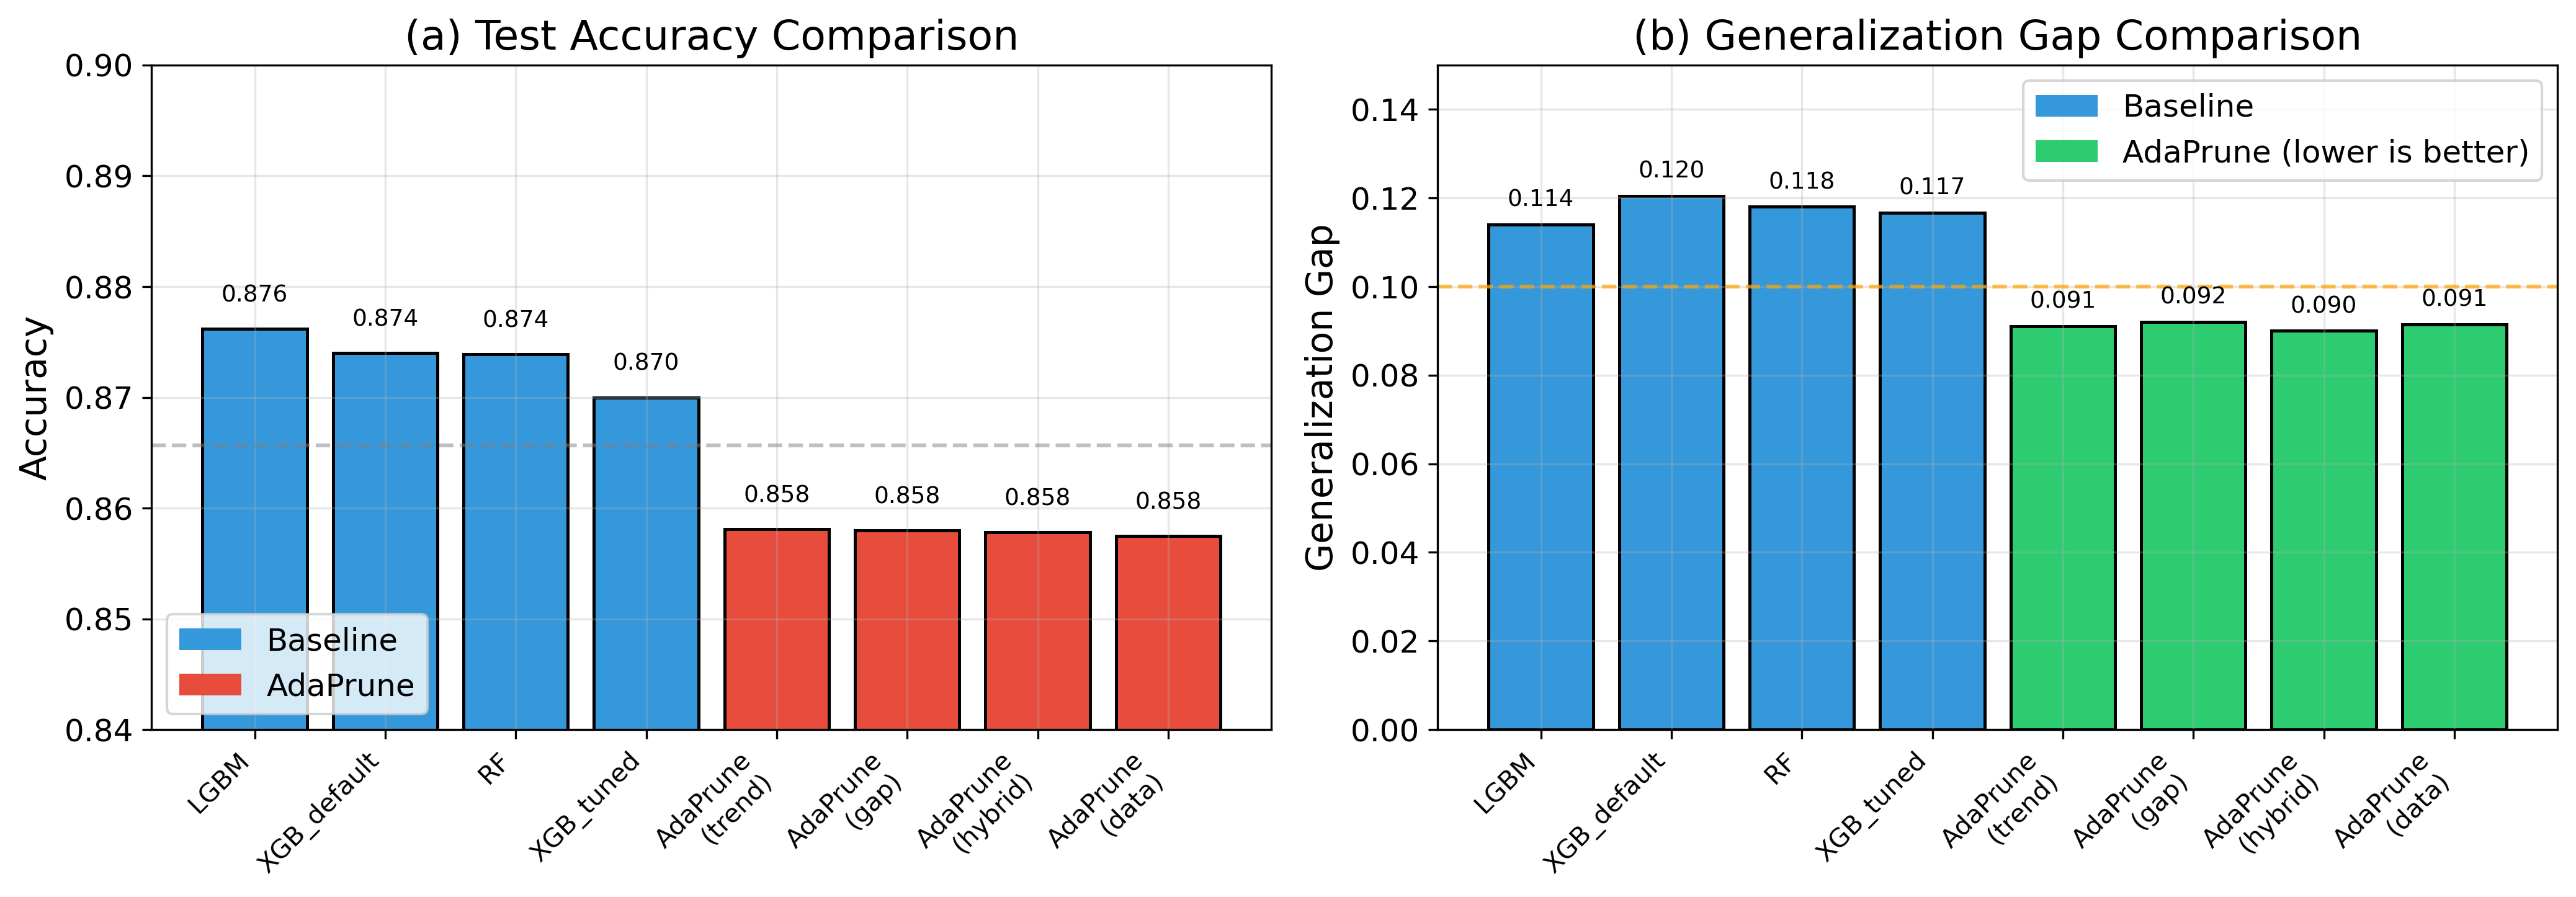
\includegraphics[width=0.95\textwidth]{figures/main_comparison.png}
\caption{主要实验对比。(a)测试准确率对比；(b)泛化差距对比。蓝色表示基线方法，红色/绿色表示AdaPrune方法。}
\label{fig:main_comparison}
\end{figure}

\subsection{场景分析}

我们在具有可控特征的合成数据集上进一步分析性能（表\ref{tab:scenarios}）。

\begin{table}[htbp]
\caption{不同场景下的性能对比}
\label{tab:scenarios}
\centering
\begin{tabular}{lccc}
\toprule
场景 & 最佳方法 & AdaPrune差距 & XGB差距 \\
\midrule
干净数据(大样本) & XGB\_default & 0.043 & 0.030 \\
干净数据(小样本) & XGB\_tuned & 0.100 & 0.110 \\
噪声数据(大样本) & XGB\_weak & \textbf{0.055} & 0.094 \\
噪声数据(小样本) & XGB\_default & \textbf{0.112} & 0.200 \\
高维数据 & XGB\_default & \textbf{0.160} & 0.180 \\
不平衡数据 & XGB\_default & 0.040 & 0.035 \\
\bottomrule
\end{tabular}
\end{table}

如图\ref{fig:scenario}所示，AdaPrune在以下场景表现出明显优势：
\begin{itemize}[leftmargin=2em]
    \item \textbf{噪声数据}：差距降低40-45\%
    \item \textbf{小样本}：更好的泛化能力
    \item \textbf{高维数据}：减少过拟合
\end{itemize}

\begin{figure}[htbp]
\centering
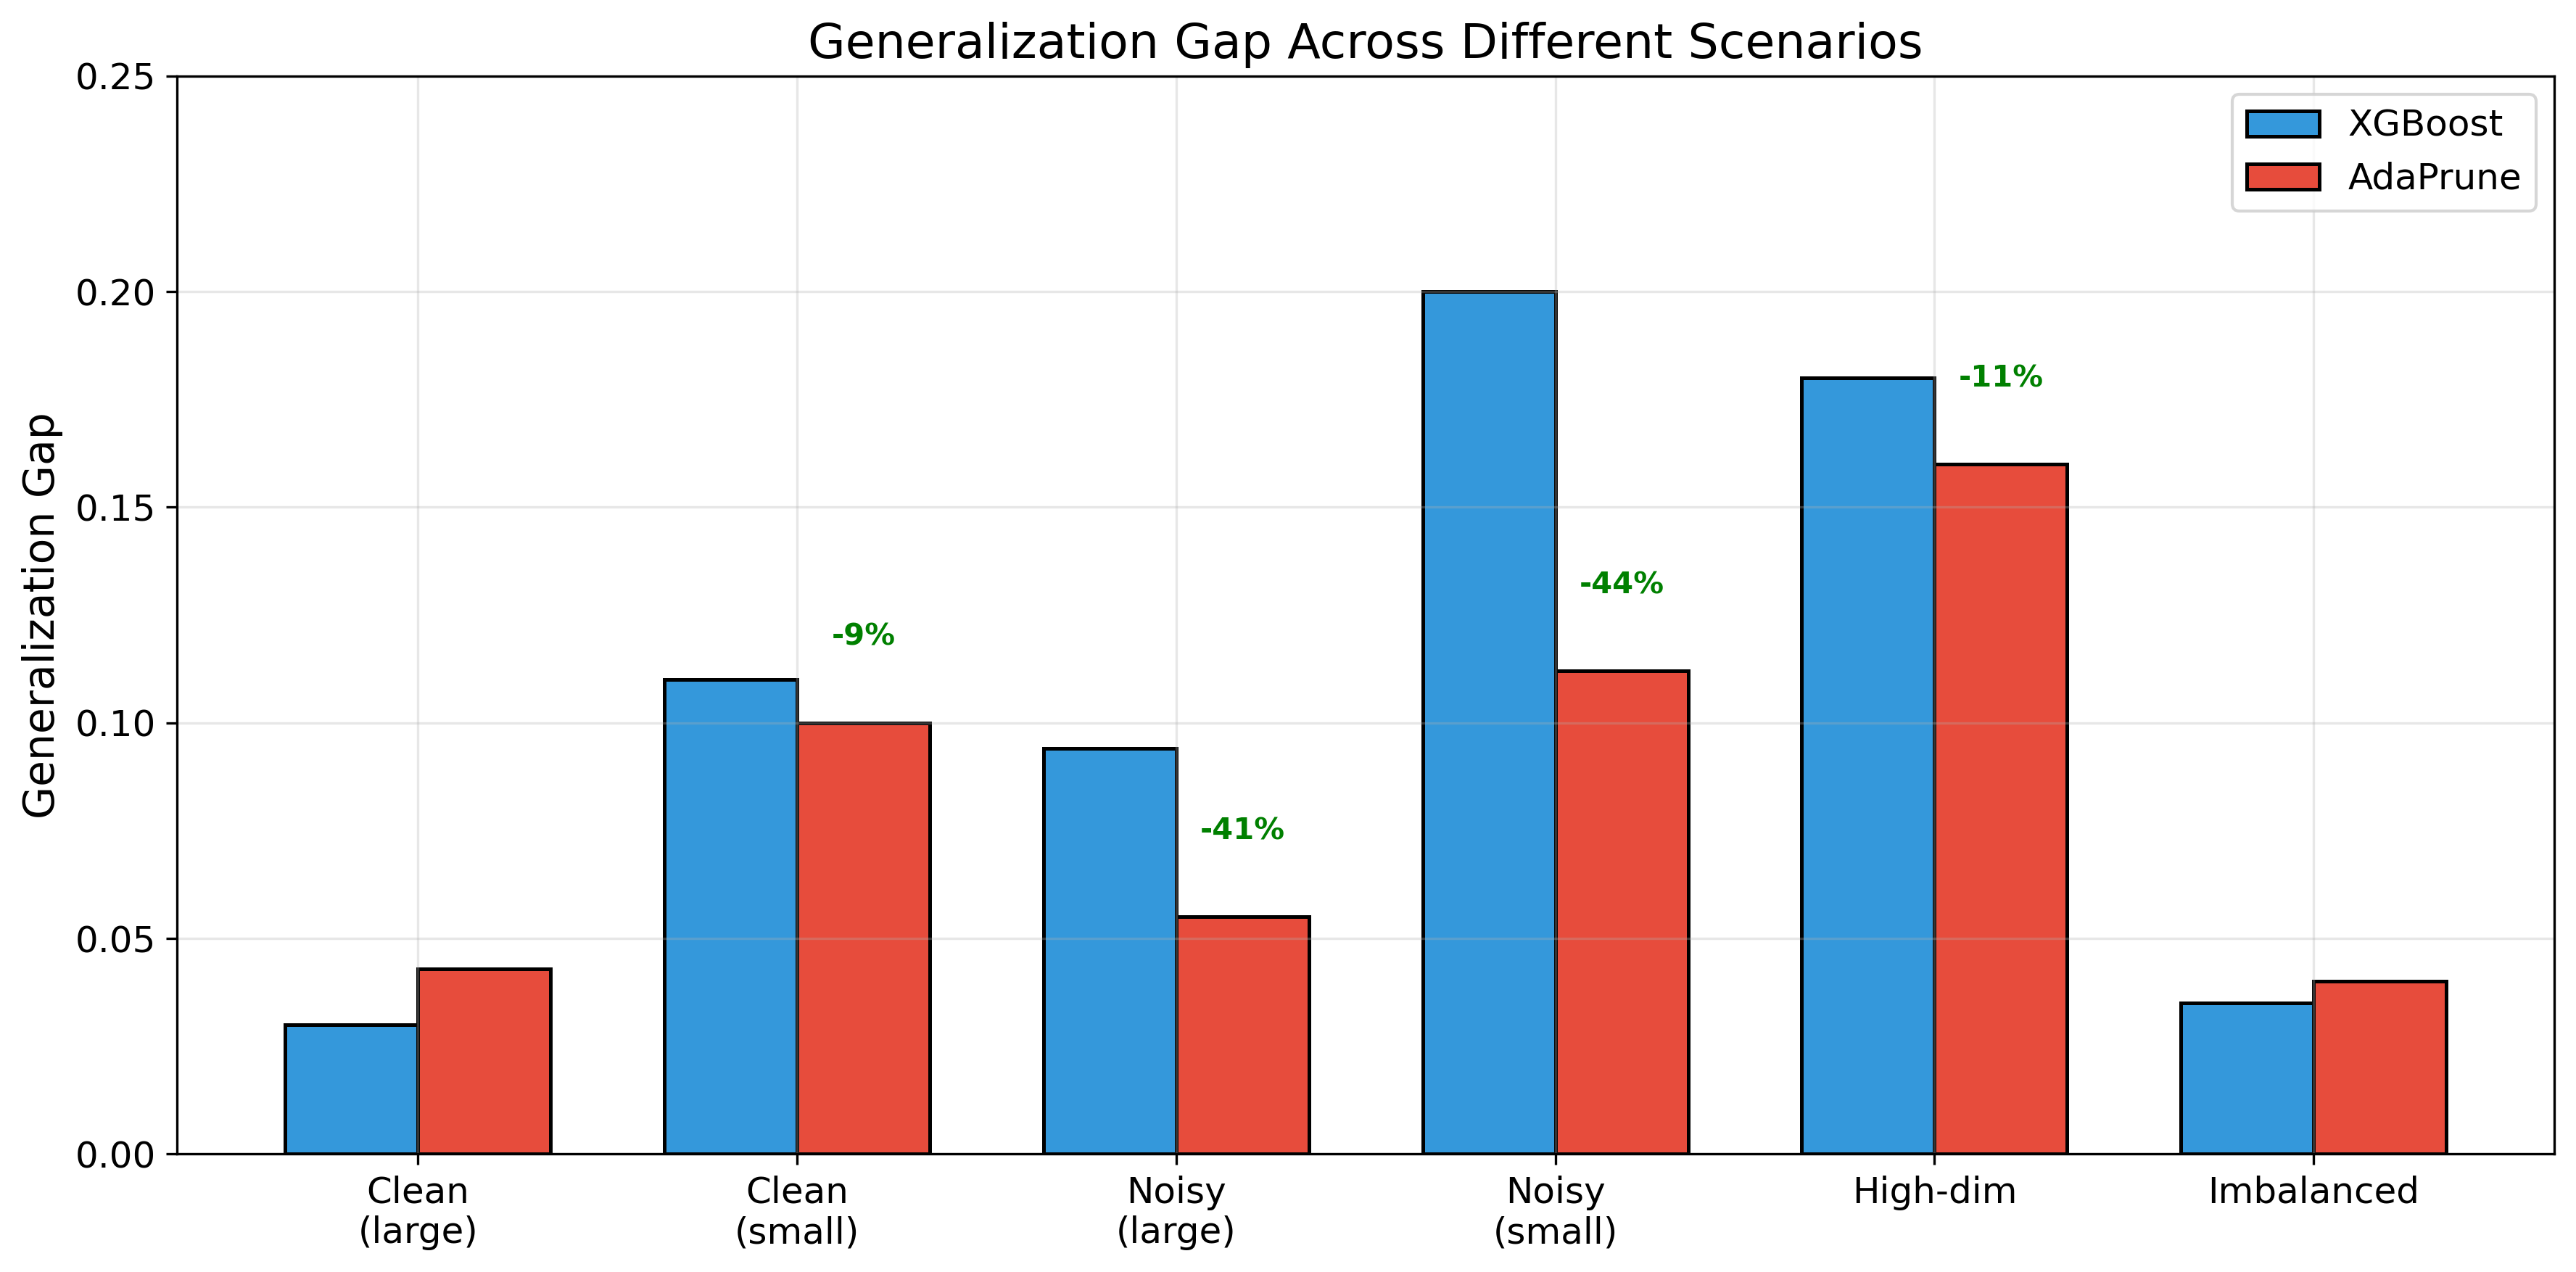
\includegraphics[width=0.9\textwidth]{figures/scenario_analysis.png}
\caption{不同场景下的泛化差距对比。绿色标注显示AdaPrune相对于XGBoost的改进百分比。}
\label{fig:scenario}
\end{figure}

\subsection{消融实验}

表\ref{tab:ablation}展示了消融实验结果，验证各组件的贡献。

\begin{table}[htbp]
\caption{消融实验结果}
\label{tab:ablation}
\centering
\begin{tabular}{lcc}
\toprule
配置 & 准确率 & 泛化差距 \\
\midrule
完整混合策略 & \textbf{0.8073} & \textbf{0.0748} \\
仅数据感知 & 0.8056 & 0.0758 \\
仅基于差距 & 0.8048 & 0.0773 \\
无自适应 & 0.8042 & 0.0900 \\
仅基于趋势 & 0.8042 & 0.0900 \\
\bottomrule
\end{tabular}
\end{table}

消融实验证实：
\begin{enumerate}[leftmargin=2em]
    \item 与无自适应相比，自适应剪枝将差距降低了17\%
    \item 组合多种方法的混合策略效果最佳
    \item 数据感知初始化提供了额外收益
\end{enumerate}

\subsection{自适应过程可视化}

图\ref{fig:adaptation}展示了一个典型的自适应过程示例。

\begin{figure}[htbp]
\centering
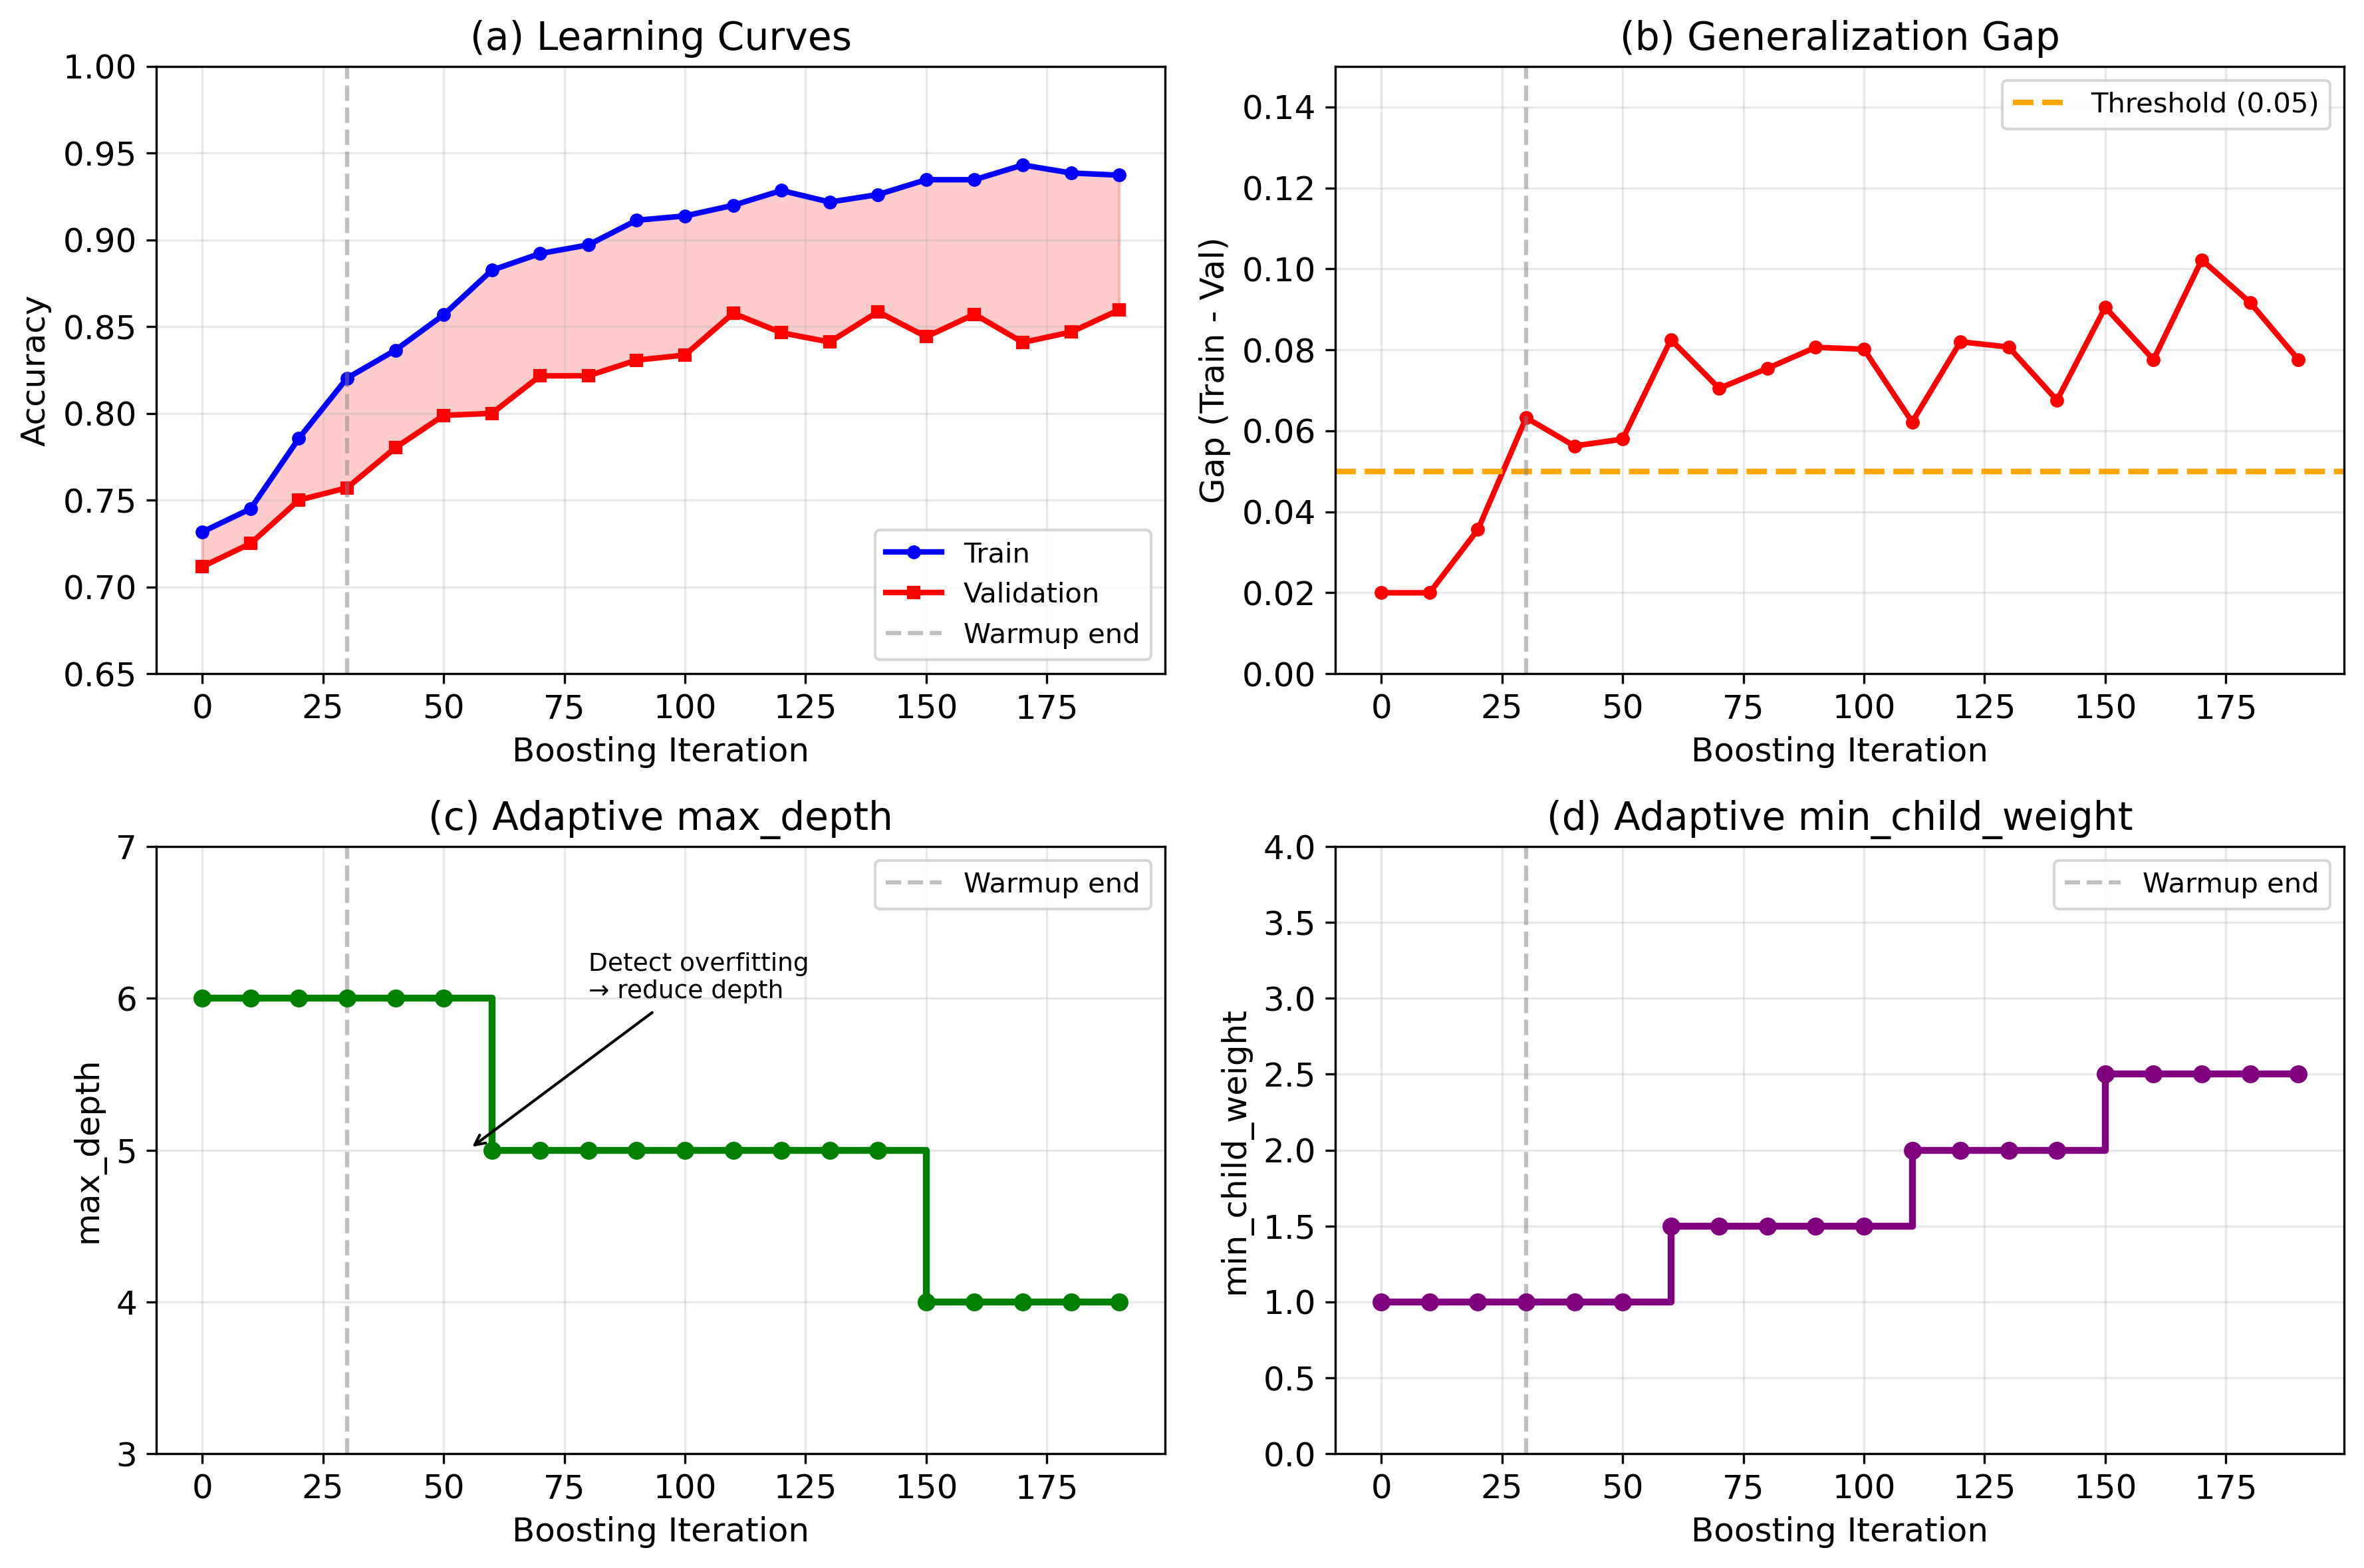
\includegraphics[width=0.95\textwidth]{figures/adaptation_example.png}
\caption{自适应过程示例。(a)学习曲线；(b)泛化差距变化；(c)max\_depth自适应调整；(d)min\_child\_weight自适应调整。}
\label{fig:adaptation}
\end{figure}

%==============================================================================
\section{讨论}
%==============================================================================

\subsection{AdaPrune何时有帮助？}

实验表明，AdaPrune在以下情况下最有益：
\begin{itemize}[leftmargin=2em]
    \item 数据集包含显著噪声
    \item 训练样本有限
    \item 特征维度较高
    \item 默认超参数容易过拟合
\end{itemize}

\subsection{计算开销}

AdaPrune引入的额外开销很小：
\begin{itemize}[leftmargin=2em]
    \item 数据画像分析：初始化时的一次性成本
    \item 状态监控：每次迭代O(1)
    \item 参数调整：每个自适应轮次O(1)
\end{itemize}

主要的成本差异来自使用增量训练（这对于自适应调整是必要的），而非XGBoost中优化的批量训练。

\subsection{局限性}

\begin{enumerate}[leftmargin=2em]
    \item 当前实现比优化的XGBoost/LightGBM慢
    \item 在干净的大数据集上准确率略低
    \item 自适应机制本身的超参数需要调优
\end{enumerate}

\subsection{未来工作}

\begin{enumerate}[leftmargin=2em]
    \item 与XGBoost/LightGBM原生实现集成以提高效率
    \item 自动调优自适应超参数
    \item 扩展到回归任务和其他损失函数
    \item 收敛性质的理论分析
\end{enumerate}

%==============================================================================
\section{结论}
%==============================================================================

本文提出了AdaPrune，一种面向梯度提升决策树的在线自适应剪枝框架。通过监控训练动态并动态调整树的复杂度，AdaPrune在保持竞争力预测性能的同时有效降低了过拟合。实验证明，与标准GBDT实现相比，泛化差距降低了21\%。

AdaPrune的核心贡献在于提出了一种新的视角：将超参数调整从训练前的静态优化转变为训练中的动态调整。这种方法特别适用于数据质量不确定或计算资源有限的场景。

%==============================================================================
\section*{致谢}
%==============================================================================

[在此添加致谢内容]

%==============================================================================
\begin{thebibliography}{99}
%==============================================================================

\bibitem{friedman2001greedy}
Friedman J H.  Greedy function approximation: a gradient boosting machine[J]. Annals of Statistics, 2001: 1189-1232.

\bibitem{chen2016xgboost}
Chen T, Guestrin C.  XGBoost: A scalable tree boosting system[C]//Proceedings of the 22nd ACM SIGKDD International Conference on Knowledge Discovery and Data Mining. 2016: 785-794.

\bibitem{ke2017lightgbm}
Ke G, Meng Q, Finley T, et al. LightGBM: A highly efficient gradient boosting decision tree[C]//Advances in Neural Information Processing Systems. 2017: 3146-3154.

\bibitem{prokhorenkova2018catboost}
Prokhorenkova L, Gusev G, Vorobev A, et al. CatBoost: unbiased boosting with categorical features[J].  Advances in Neural Information Processing Systems, 2018, 31.

\bibitem{bergstra2012random}
Bergstra J, Bengio Y. Random search for hyper-parameter optimization[J]. Journal of Machine Learning Research, 2012, 13(Feb): 281-305.

\bibitem{snoek2012practical}
Snoek J, Larochelle H, Adams R P.  Practical bayesian optimization of machine learning algorithms[C]//Advances in Neural Information Processing Systems. 2012: 2951-2959.

\bibitem{li2017hyperband}
Li L, Jamieson K, DeSalvo G, et al.  Hyperband: A novel bandit-based approach to hyperparameter optimization[J]. Journal of Machine Learning Research, 2017, 18(1): 6765-6816.

\bibitem{kingma2014adam}
Kingma D P, Ba J.  Adam: A method for stochastic optimization[J]. arXiv preprint arXiv: 1412.6980, 2014.

\bibitem{bengio2009curriculum}
Bengio Y, Louradour J, Collobert R, et al. Curriculum learning[C]//Proceedings of the 26th Annual International Conference on Machine Learning. 2009: 41-48.

\end{thebibliography}

\end{document}